\chapter{Análisis Teórico-Computacional de la propuesta de solución. Detalles de implementación}\label{chapter:proposal}
En el capítulo anterior se realizó un análisis del estado del arte, concluyendo con la
necesidad de implementar desde cero una aplicación de Android usando Flutter para su desarrollo, que cumpla con los requerimientos planteados.
Este capítulo estará enfocado en el marco teórico-computacional de la propuesta de
solución para este proyecto. Se abordarán temas que incluyen los detalles de la arquitectura seleccionada, la modelación de los datos del problema
y el análisis de los requerimientos funcionales de la aplicación. Se abordarán también las principales tecnologías utilizadas, así como, algunos detalles de implementación.
\section{Diagrama de casos de uso}
En esta sección se expondrán las acciones que puede realizar un usuario dentro de la aplicación, explicado a través de un diagrama de casos de uso
\footnote{Diagrama de casos de uso: Forma de diagrama de comportamiento UML(Unified Modeling Language o en español Lenguaje de Modelado Unificado) mejorado. Sirve para
    especificar la comunicación y el comportamiento de un sistema mediante su interacción con los usuarios
    y/u otros sistemas. Un diagrama que muestra la relación entre los actores y los Casos de Uso en un
    sistema.}
, teniendo en cuenta que solo existe un rol de usuario, Encuestador,
y tres grupos de acciones que se encapsulan en el diagrama por comodidad para el lector, Acciones de importación/exportación, Acciones en la pestaña "Mapa" y Acciones en
la pestaña "Registro".
\pagebreak
\begin{figure}[h]
    \centering
    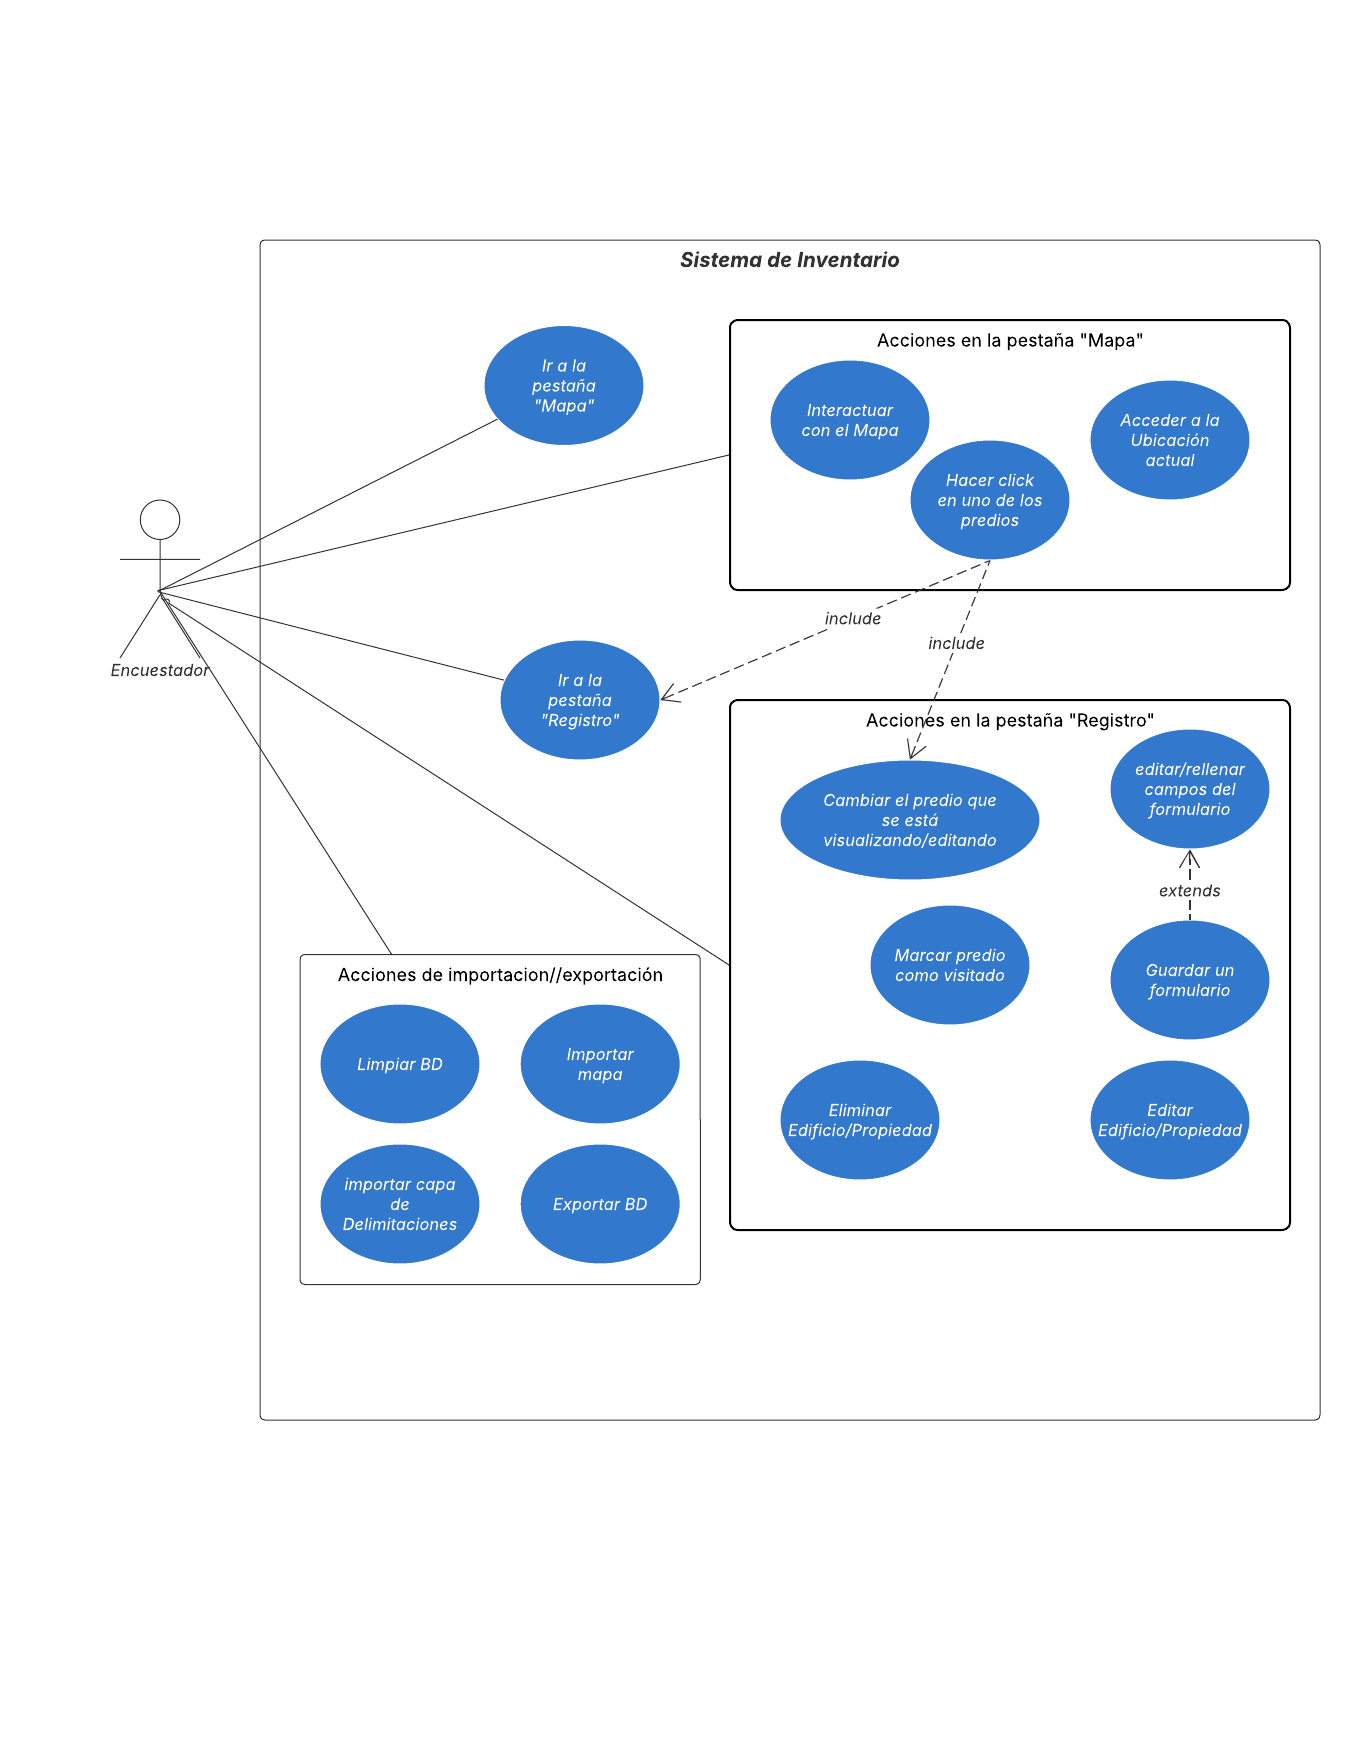
\includegraphics[scale=0.5]{Graphics/Capitulo 3/Diagrama_casos_de_uso.png}
    \caption{Diagrama de casos de uso de la aplicación Inventario.} % Título de la figura
    \label{fig:figura13}
\end{figure}
En la figura anterior(Ver figura \ref{fig:figura13}) se puden observar las diversas acciones que puede realizar un encuestador dentro de
la aplicación. Las mismas se explican a continuación:
\begin{itemize}
    \item \textbf{Ir a la pestaña "Mapa"}: Al presionar en la pestaña nombrada de esta manera se abrirá la vista de Mapa. Por defecto esta es la vista que se muestra.
    \item \textbf{Ir a la pestaña "Registro"}: Al presionar en la pestaña nombrada de esta manera se abrirá la vista de Registro o Formulario. Aquí se podrá introducir información relacionada con los predios, edificios y propiedades que se deseen.
    \item \textbf{Acciones de importación/exportación}
          Aqui se debe recalcar que estas funcionalidades diseñadas puramente por comodidad para los encuestadores, ya que se se colocan el mapa y las
          delimitaciones que se quieren mostrar, en las carpetas correspondientes no será necesario usar más nada, se mostrarán automáticamente en la aplicación.
          \begin{itemize}
              \item \textbf{Importar Mapa}: Esta opción abrirá una nueva ventana de selección de archivos, donde el usuario deberá seleccionar
                    un archivo con extensión ".mbtiles" para importarlo en la aplicación. Esto realizará una copia del archivo seleccionado hacia
                    la carpeta de mapas de la aplicación en el almacenamiento del dispositivo('CADIC/Maps'). Para que la importación surta efecto,
                    se deberá cambiar rápidamente de pestaña o cerrar y abrir la aplicación.
              \item \textbf{Importar capa de Delimitaciones}: También abrirá una ventana de selección de archivos, pero esta vez esperando que
                    el usuario localice un archivo con extensión ".geojson". Dentro del archivo deben encontrarse definiciones de polígonos, y
                    dentro de cada polígono, en el apartado de "properties" podrá incluirse la etiqueta individual que se deseará mostrar para
                    cada polígono, esta se mostrará en el centro de cada polígono al renderizarse en el mapa. En el caso de una capa de polígonos
                    que representen predios, el archivo que contiene las delimitaciones deberá cumplir 2 resticciones para obtener
                    una correcta integración y funcionamiento con la aplicación. Una de estas restricciones es que el nombre termine de la siguiente manera:
                    \begin{mdframed}
                        (...)\_predios.geojson
                    \end{mdframed}
                    Por ejemplo: "managua\_predios.geojson". La otra restricción es que cada definición de polígono interna en el archivo,
                    tenga una propiedad "localizacion" (sin tilde), con valor igual al número de localización correspondiente al predio que define.
                    De esta manera se importarán correctamente las delimitaciones, considerando cada archivo como una capa, y pintando de un color
                    diferente cada una de estas capas.

              \item \textbf{Exportar BD}: Esto exportará la BD hacia el directorio 'CADIC/Exportado'.
              \item \textbf{Limpiar BD}: Limpia la Base de Datos, solo dejando el nombre del encuestador registrado al iniciar la aplicación por primera vez.
          \end{itemize}
    \item \textbf{Acciones en la pestaña "Mapa"}
          \begin{itemize}
              \item \textbf{Interactuar con el mapa}: En la pestaña "Mapa", la funcionalidad primaria es la interacción con el mapa, lo que abarca desde
                    el acercamiento/alejamiento de la vista del mapa, como el desplazamiento de la vista horizontal y verticalmente. Esto se realiza con
                    los gestos clásicos de navegación por el mapa sobre la pantalla táctil del dispositivo.
              \item \textbf{Hacer click en uno de los predios}: Al cargar las delimitaciones de los predios, edificios y manzanas sobre el mapa,
                    los predios no solo se deberían mostrar como polígonos con borde de color rojo, sino que también deberán tener un marcador visualizado
                    como punto de color negro en su centroide. Al hacer click sobre uno de estos puntos en el mapa, automáticamente se accederá a la información
                    registrada del predio asociado al marcador, abriéndose la vista de la pestaña "Registro" con los datos del predio si había sido registrado previamente.
                    \footnote{El centroide, también conocido como baricentro, es el centro geométrico de una figura o cuerpo. Representa el punto donde se concentraría toda
                        la masa si el objeto tuviera una distribución uniforme de masa. En otras palabras, es el punto de equilibrio de la figura. }

              \item \textbf{Acceder a la ubicación actual}: Si se presiona sobre el botón con un ícono de objetivo, la vista del mapa se centrará en
                    la localización actual del usuario.
          \end{itemize}
    \item \textbf{Acciones en la pestaña "Registro"}
          \begin{itemize}
              \item \textbf{Cambiar el predio que se está visualizando/editando}: Por defecto en la vista del Formulario, el número de Localización no se puede variar,
                    pero al lado de este campo inhabilitado, se encontrará una casilla para marcar, la cuál si está en efecto marcada, permitirá cambiar el número de
                    localización, lo que concede acceder manualmente a la información de un predio con solo introducir su identificador de localización.
              \item \textbf{Editar/rellenar campos del formularios}: Sin profundizar aún mucho en el tema, cabe mencionar que los formularios son reactivos, y por lo tanto,
                    varias acciones que se realicen en la aplicación, tendrán repercución en lo que se muestra y lo que no del formulario.
              \item \textbf{Guardar un formulario}: Un formulario no se registrará en la Base de Datos si no se presiona el botón de "Guardar"
              \item \textbf{Editar edificio/propiedad}: Si el número de localización actual del formulario, refiere a un predio ya registrado en la base de datos, en caso de
                    que este predio tenga edificios ya registrados, igualmente se mostrarán en una lista de elementos visuales dentro del subformulario Edificio. Luego, la manera
                    de editar un edificio ya existente, es presionando sobre el elemento visual que lo identifica con una letra 'E' acompañada de su número de edificio. Esta cambiará
                    de color y de esta manera se sabrá que este edificio está siendo editado. Los campos que hayan sido rellenados previamente del edificio se visualizarán por si se
                    desea editarlos. \\
                    Un comportamiento similar ocurre con la relación edificio-propiedades. Cuando un edificio esté seleccionado, y se aprecie con un color verde claro, como
                    anteriormente se dijo, este está seleccionado, esto significa que se podrá editar y al mismo tiempo el formulario mostrará un nuevo subformulario "Propiedades"
                    que mostrará las propiedades asociadas al edificio seleccionado, como una lista de elementos visuales que representan a cada propiedad mostrando una letra "P" junto
                    al Número de local de cada propiedad, de manera similar a como lo hace el subformulario "Edificio" con los edificios del predio seleccionado.
                    Para editar una propiedad se hará igual a como se edita un edficio, presionando encima del elemento visual que la identifica. De igual manera al hacer esto, el elemento visual
                    presionado cambiará a un color verde claro, indicando que la propiedad que representa está siendo editada, mostrando en el subformulario Propiedad los valores guardados
                    de la propiedad en cuestión para cada campo.
              \item \textbf{Eliminar edificio/propiedad}: A la derecha de cada elemento visual que representa tanto una propiedad como los de cada edificio, se observará una pequeña cruz
                    la cuál al ser presionada hará que se elimine dicha propiedad o dicho edificio respectivamente. Luego de haber eliminado la entidad en cuestión, en caso de haber presionado
                    esta opción por error, será posible revertir esto antes de los 5 segundos de haber eliminado la entidad presionando "Deshacer" en una barra auxiliar que aparecerá justo luego de
                    haber eliminado.
              \item \textbf{Marcar predio como visitado}: Esta es una de las funcionalidades más útiles visualmente para un encuestador al estar en una inspección. Al final del formulario en la pestaña
                    de Registro, habrá un botón con el texto "Predio Visitado"; al presionarlo, este hará que visualmente el predio en cuestión cambie de color en sus border, o sea, que se coloree
                    de verde, y que se rellene con un color verde un poco mas claro y con tono trasparente. Esto será una herramienta que se use meramente por comodidad, no se guardará información
                    referente a este cambio en la Base de Datos ni en los archivos de delimitaciones.
          \end{itemize}

\end{itemize}
\section{Propuestas de Arquitectura}
Luego de investigar varias arquitecturas propicias para el desarrollo en Flutter, valorarlas y pensar en cuál sería la ideal para un proyecto no tan grande,
teniendo en cuenta arquitecturas modernas y otras no tan modernas pero utilizadas comúnmente en proyectos de Flutter, se llegó a la conclusión de que se utilizaría
una arquitectura Modelo-Vista-Modelo de Vista (MVVM por sus siglas en inglés)\cite{MVVM}, una variación moderna de la arquitectura Modelo-Vista-Controlador(MVC) \cite{MVC},
con ciertos ajustes y adaptaciones mínimas dado el corto tiempo del que se dispone y los patrones de desarrollo y arquitectura de Flutter en si.
\subsection{Aruitectura Modelo-Vista-Modelo de Vista}
El patrón MVVM fue introducido por John Gossman en 2005 mientras trabajaba en Microsoft, y fue diseñado inicialmente para su uso
con Windows Presentation Foundation (WPF) y Silverlight. Desde entonces, MVVM ha sido adoptado en diversas plataformas y frameworks como Flutter,
debido a sus beneficios en la separación de responsabilidades y la mejora de la testabilidad.
Este patrón de arquitectura o simplemente arquitectura, busca separar estrictamente la Interfaz de usuario de la lógica de negocio y de presentación, estableciendo un componente
intermedio como lo hace la arquitectura MVC con el Controlador, pero en este caso con el Modelo de Vista o ModelView. La principal diferencia entre estas dos arquitecturas
es que en MVC se trata de separar el acceso a los datos mediante el componente Controlador, pero en MVVM se trata de separar la lógica de negocio de la UI a través del componente
Modelo de Vista, el cuál mantendrá el estado de los datos que se muestran en la Vista y será reactivo al cambio de la misma, haciendo variaciones internas y dejando los datos en
un formato listo para ser mostrado nuevamente, dejando la responsabilidad de los datos en si y el acceso a ellos, al componente Modelo, por lo que esta arquitectura está orientada
a la claridad y limpieza de la Vista o UI. Por lo que, resumiento las resposabilidades de cada componente de esta arquitectura, estas son:

\begin{itemize}
    \item \textbf{Modelo}: Contiene las entidades de dominio (datos). Contiene las reglas de negocio. Accede a bases de datos, servicios remotos, etc.
    \item \textbf{Vista}: Solo se encarga de mostrar datos. Observa al ViewModel. Notifica al ViewModel de los eventos de usuario.
    \item \textbf{Modelo de Vista}:
          \begin{itemize}
              \item Contiene la lógica de presentación.
              \item Expone los datos a la vista en un formato listo para mostrar.
              \item Responde a eventos de la vista.
              \item Hace la comunicación con el modelo.
              \item Maneja el estado de la vista.
              \item No tiene referencia directa a la vista.
          \end{itemize}

\end{itemize}
\subsection{Arquitectura MVVM aplicada a la propuesta de solución}
En la siguiente imagen se muestra la estructura del proyecto:
\begin{figure}[h]
    \centering
    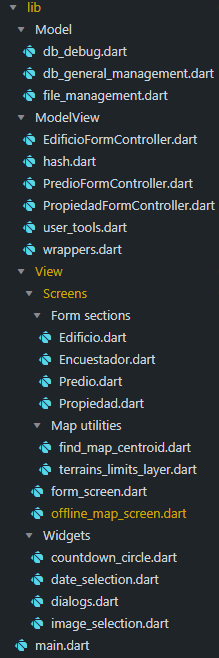
\includegraphics[scale=0.5]{Graphics/Capitulo 3/estructura_del_codigo.png}
    \caption{Estructura del código.} % Título de la figura
    \label{fig:figura14}
\end{figure}

En la figura anterior (Ver figura \ref{fig:figura14})se pueden apreciar las diferentes capas de la arquitectura MVVM bien definidas,
representadas por las carpetas "Model", "View" y "ViewModel" que contienen la parte del código relacionada con la capa de arquitectura
que su nombre indica:\\\\
\textbf{Model}
Aquí se encuentra la capa que abarca los datos y el acceso a ellos. Se hace uso de la librería sqflite \cite{sqflite} como mediador de comunicación
con bases de datos SQLite. Se encierra el modelo de datos en una jerarquía de clases reutilizable y expandible que tiene como padre la clase abstracta "DBTable",
de la cuál las clases que representan las tablas del modelo de datos del problema heredan, obligándoles a implementar propiedades y métodos que proporcionarán
el formato de los datos que requiere sqflite para insertar en sus tablas correspondientes. Estas clases asociadas a las tablas de la Base de Datos
son "Predio", "Edificio" y "Propiedad".
\\
\textbf{View}
El componente Vista está dividido en dos partes, las pantallas o "Screens" y los "Widgets"
\footnote{Los widgets son básicamente componentes de Flutter utilizados para crear la interfaz de usuario de
    la aplicación}.
Existen solo dos pantallas en este caso, la pantalla del mapa sin conexión, que es donde se hace uso de las librerías flutter\_map y flutter\_map\_mbtiles para
obtener el componente que renderiza el mapa a partir de un archivo con formato/extensión ".mbtiles", y la pantalla del formulario, donde se hace uso de la gran.
\\
\textbf{ModelView}
\\
\section{Modelo de Base de Datos}
\subsection{Predio}
\subsection{Edificio}
\subsection{Propiedad}
\section{Tecnologías y librerías utilizadas}
\section{Detalles de implementación}
\subsection{Subformularios }
\subsection{Reactividad de los formularios}
\subsection{Validación de formularios}
\subsection{Restricciones y visibilidad de campos de los formularios}
\subsection{Exportación e importación de archivos}
\subsection{Extensión del código}
\section{Conclusiones del capítulo}